\documentclass[paper=a4, DIV=100]{scrbook}
\usepackage{tikz}
\usepackage{setspace}
\usepackage{fontspec}
\setmainfont{Minion Pro}

\title{Unmasking the Gamma-Ray Sky}
\subtitle{Comprehensive and Reproducible Analysis for Cherenkov Telescopes}
\author{Kai Brügge}

\begin{document}
\begin{titlepage}
    % \tikz[remember picture,overlay] \node[opacity=0.2,inner sep=0pt] at (current page.center){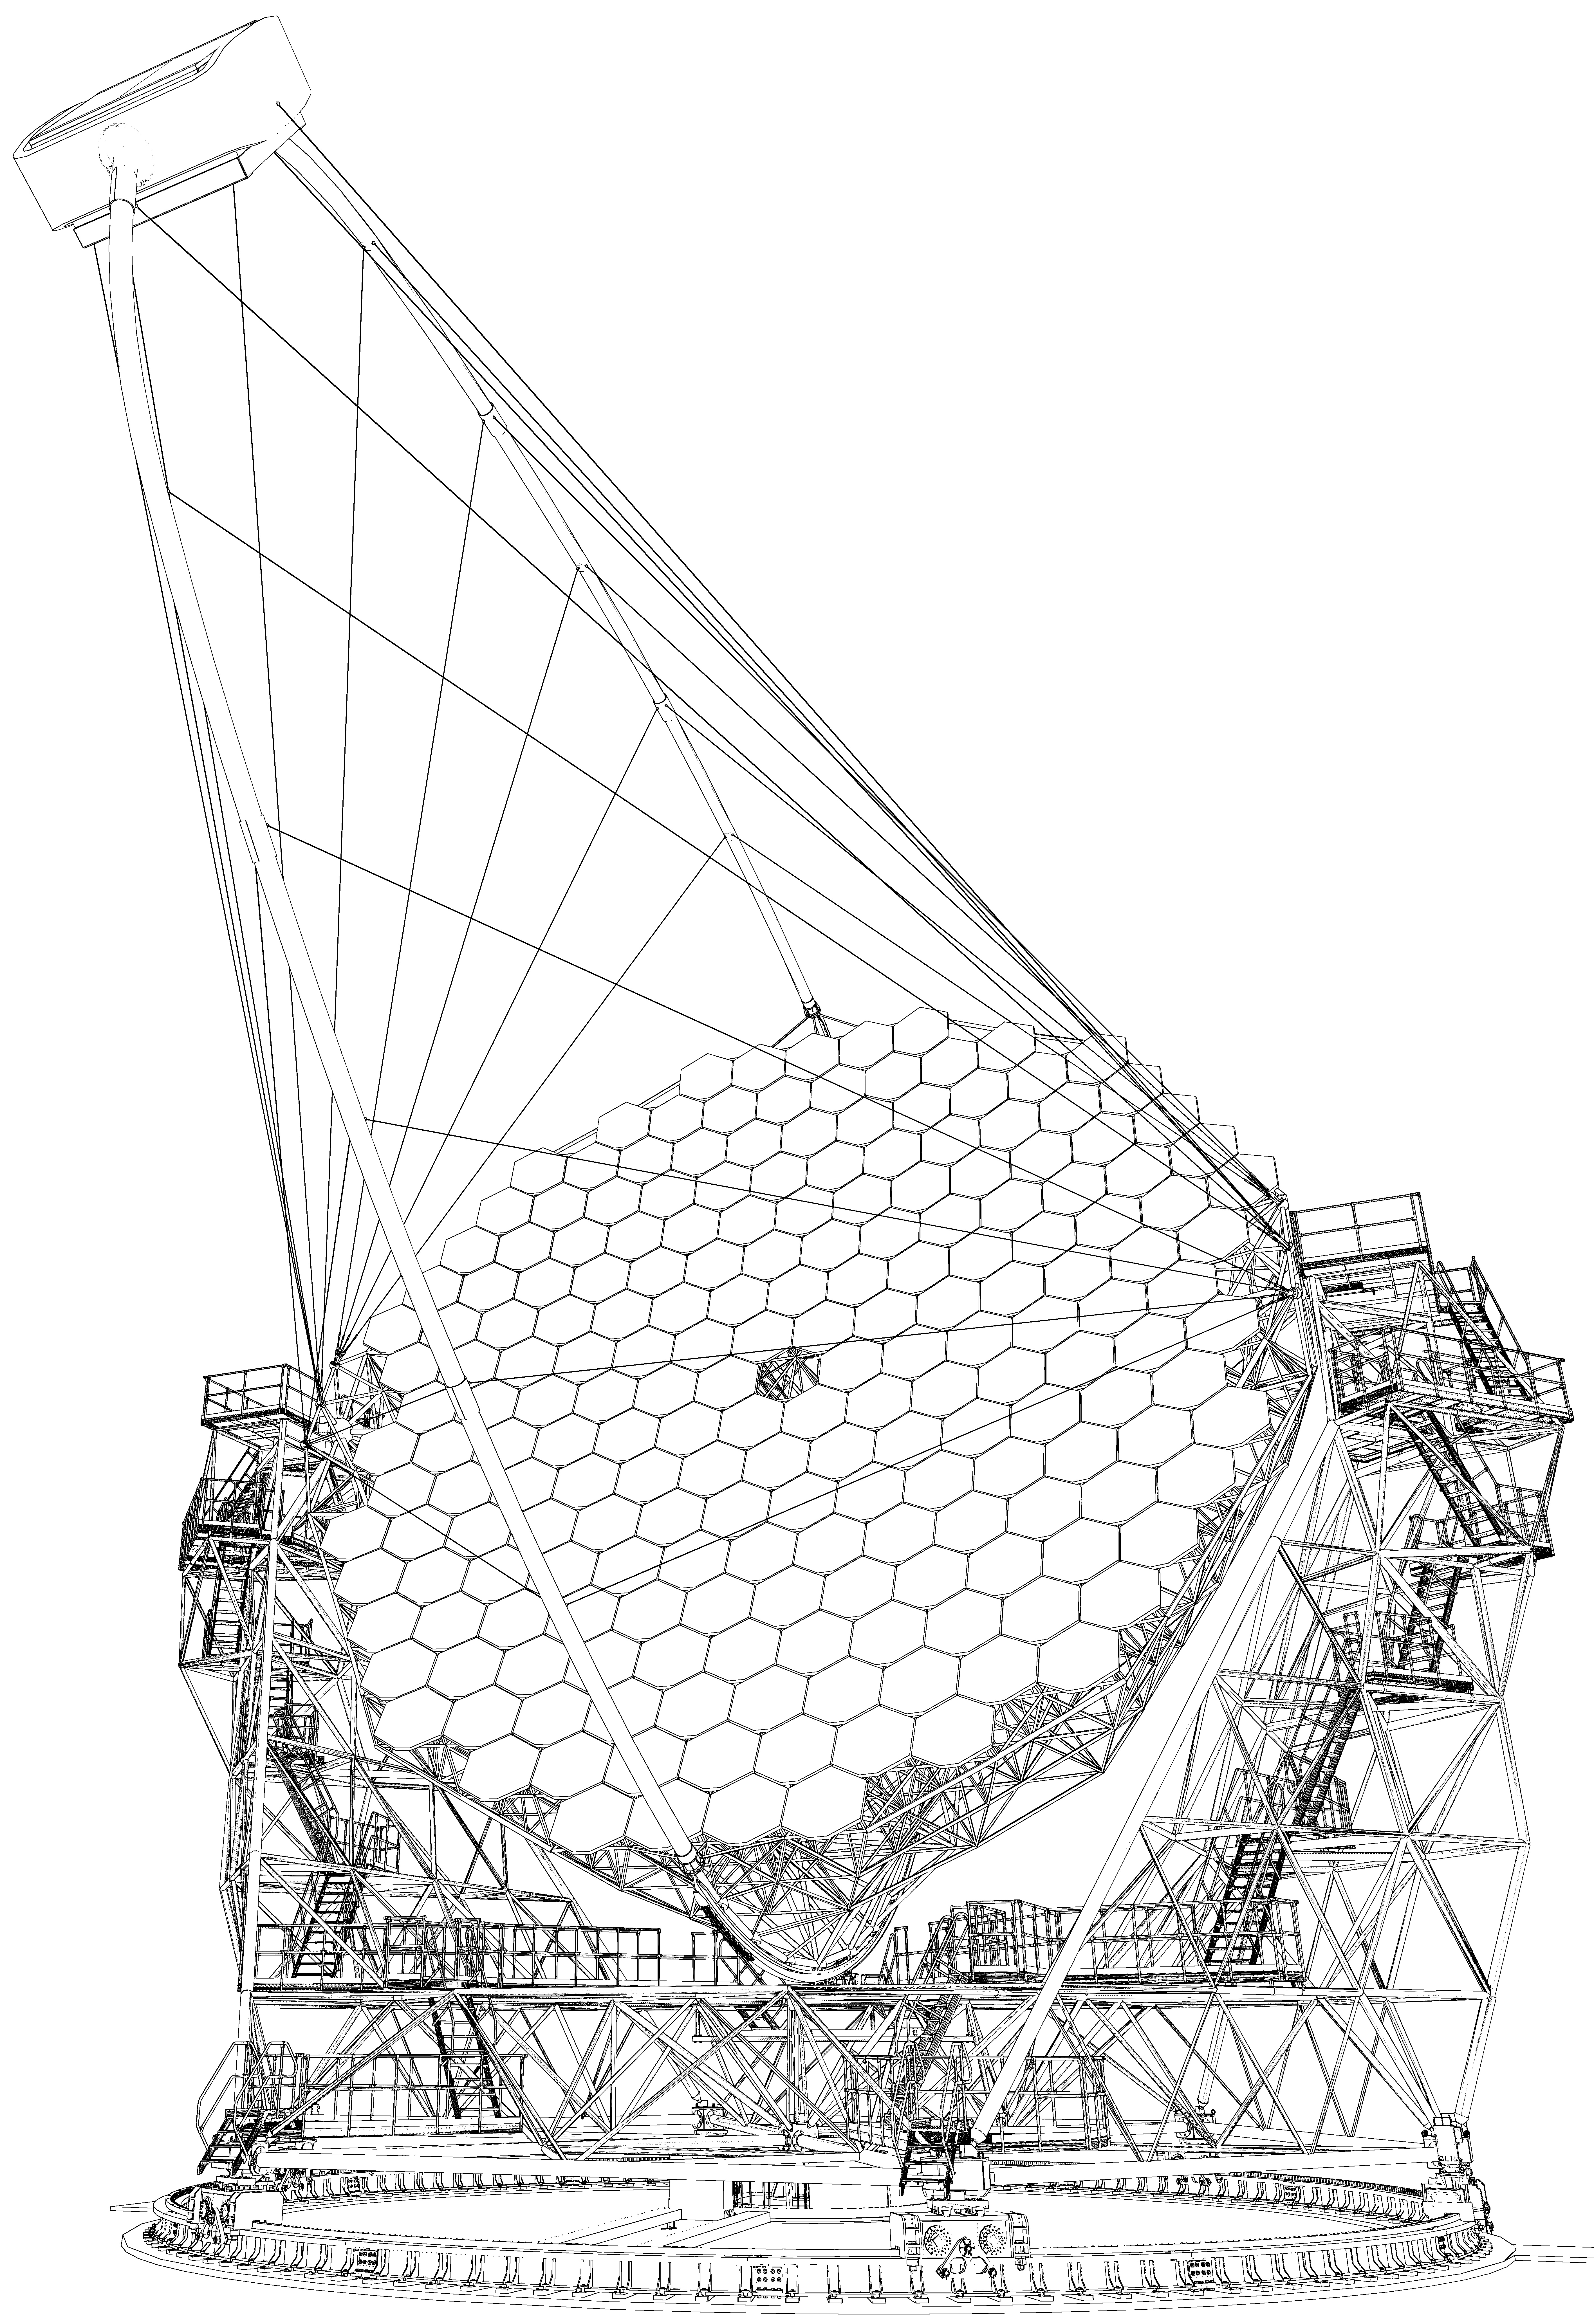
\includegraphics[width=\paperwidth,height=\paperheight]{figures/contours_lst.jpg}};%
    \tikz[remember picture,overlay] \node[inner sep=10pt, anchor=north east] at (current page.north east){\hspace{-25em}\includegraphics[width=0.4\paperwidth]{figures/tudo_logo.jpg}};%
    \vspace*{10cm}
    \makeatletter
    \begin{center}
    {\setstretch{1.2}
            
    \KOMAoption{fontsize}{32pt}
        \@title
    \\[0.5cm]
      %
      \KOMAoption{fontsize}{12pt}
      \begin{Large}
        \@subtitle
      \end{Large}\\
      %
      % \emph{by}\\
      % \@author
      %
      % \vspace{10cm}
      
      % A document submitted in partial fulfillment
      % of the requirements for the degree of\\
      % \emph{Dr. rer. nat.}\\
      % at\\
      % \textsc{Technische Universität Dortmund}
      
      \vspace{13.cm}
      % Dissertation \\
      % \emph{by}\\
      \begin{Large}
        Kai Brügge \\
        \vspace{0.1cm}
        2019
      \end{Large}
      % Supervis`ed by \\
    % Prof.\,Dr.\,Dr.\,Wolfgang Rhode\,  and\,   Prof.\,Dr.\,Kevin Kröninger

    \par}

    \end{center}
    
    \makeatother
  \end{titlepage}

\end{document}